\documentclass[10pt,twocolumn]{article} 
\usepackage{simpleConference}
\usepackage{times}
\usepackage{graphicx}
\usepackage{amssymb}
\usepackage{url,hyperref}

\begin{document}

\title{\LaTeX\ Template for a Simple, Two-Column Paper}

\author{Iroro Orife \\
\\
Technical Report \\
Seattle, Washington, USA \\
\today
\\
\\
iroro@alumni.cmu.edu  \\
}

\maketitle
\thispagestyle{empty}

\begin{abstract}
The material in this template is an edited \& \LaTeX\--ified version of the recommendations here: \url{http://cs.stanford.edu/people/widom/paper-writing.html} The objective would be to help us writers, stay on topic and focused for each section of a report.

For the abstract state the problem, your approach and solution, and the main contributions of the paper. Include little if any background and motivation. Be factual but comprehensive. The material in the abstract should not be repeated later word for word in the paper. 
\end{abstract}


\section{Introduction}
The Introduction is crucially important. By the time a referee has finished the Introduction, he's probably made an initial decision about whether to accept or reject the paper. He'll read the rest of the paper looking for evidence to support his decision. A casual reader will continue on if the Introduction captivated him, and will set the paper aside otherwise. 
Here is the Stanford InfoLab's patented five-point structure for Introductions. Unless there's a good argument against it, the Introduction should consist of five paragraphs answering the following five questions:

\begin{description}
  \item[$\bullet$]  What is the problem?
  \item[$\bullet$]  Why is it interesting and important?
  \item[$\bullet$]  Why is it hard? Why do naive approaches fail?
  \item[$\bullet$]  Why hasn't it been solved before? What's wrong with previous proposed solutions? How does mine differ?
  \item[$\bullet$]  What are the key components of my approach and results? Also include any specific limitations.
\end{description}
  
Then have a final paragraph or subsection: ``Summary of Contributions". It should list the major contributions in bullet form, mentioning in which sections they can be found. This material doubles as an outline of the rest of the paper, saving space and eliminating redundancy.

\section{Related Work}

The perennial question: Should related work be covered near the beginning of the paper or near the end?

\begin{description}
  \item[$\bullet$]  Beginning, if it can be short yet detailed enough, or if it's critical to take a strong defensive stance about previous work right away. In this case Related Work can be either a subsection at the end of the Introduction, or its own Section 2.
  \item[$\bullet$]  End, if it can be summarized quickly early on (in the Introduction or Preliminaries), or if sufficient comparisons require the technical content of the paper. In this case Related Work should appear just before the Conclusions, possibly in a more general section ``Discussion and Related Work".
\end{description}

\section{The Body}

\textbf{Guideline 1:} A clear new important technical contribution should have been articulated by the time the reader finishes page 3 i.e., a quarter of the way through the paper.

\textbf{Guideline 2:} Every section of the paper should tell a story. Don't, however, fall into the common trap of telling the entire story of how you arrived at your results. Just tell the story of the results themselves. The story should be linear, keeping the reader engaged at every step and looking forward to the next step. There should be no significant interruptions -- those can go in the Appendix.
\\
\\
Aside from these guidelines, which apply to every paper, the structure of the body varies a lot depending on content. Important components are:

\begin{description}
  \item[$\bullet$]  Running Example: When possible, use a running example throughout the paper. It can be introduced either as a subsection at the end of the Introduction, or its own Section 2 or 3 (depending on Related Work).
  \item[$\bullet$]  Preliminaries: This section, which follows the Introduction and possibly Related Work and/or Running Example, sets up notation and terminology that is not part of the technical contribution. One important function of this section is to delineate material that's not original but is needed for the paper. Be concise -- remember Guideline 1.
    \item[$\bullet$] Content: The meat of the paper includes algorithms, system descriptions, new language constructs, analyses, etc. Whenever possible use a ``top-down" description: readers should be able to see where the material is going, and they should be able to skip ahead and still get the idea.
\end{description}


\section{Performance Experiments}

We could have an entire treatise on this topic alone and I am surely not the expert. Here are some random thoughts:

\begin{description}
  \item[$\bullet$]  Many conferences expect experiments.
  \item[$\bullet$]  It's easy to do ``hokey" or meaningless experiments, and many papers do.
  \item[$\bullet$]  It's easy to craft experiments to show your work in its best light, and most papers do.
    \item[$\bullet$]  What should performance experiments measure? Possibilities:  
    \begin{description}
  	  \item[$\bullet$] Pure running time
      \item[$\bullet$] Sensitivity to important parameters
      \item[$\bullet$] Scalability in various aspects: data size, problem complexity, ...
  \end{description}
    \item[$\bullet$]  What should performance experiments show? Possibilities:
        \begin{description}
  	  \item[$\bullet$] Absolute performance i.e., it's acceptable/usable
      \item[$\bullet$] Relative performance to naive approaches
      \item[$\bullet$] Relative performance to previous approaches
      \item[$\bullet$] Relative performance among different proposed approaches
  \end{description}
  \item[$\bullet$] 
\end{description}


\section{The Conclusions}

In general a short summarizing paragraph will do, and under no circumstances should the paragraph simply repeat material from the Abstract or Introduction. In some cases it's possible to now make the original claims more concrete, e.g., by referring to quantitative performance results.

\section{Future Work}

This material is important -- part of the value of a paper is showing how the work sets new research directions. I like bullet lists here. A couple of things to keep in mind:
\begin{description}
  \item[$\bullet$]  If you're actively engaged in follow-up work, say so. E.g.: ``We are currently extending the algorithm to... blah blah, and preliminary results are encouraging." This statement serves to mark your territory.
\item[$\bullet$]  Conversely, be aware that some researchers look to Future Work sections for research topics. My opinion is that there's nothing wrong with that -- consider it a compliment.
\end{description}

\section{The Acknowledgements}

Don't forget them or you'll have people with hurt feelings. Acknowledge anyone who contributed in any way: through discussions, feedback on drafts, implementation, etc. If in doubt about whether to include someone, include them.


\section{Citations}

Spend the effort to make all citations complete and consistent. Do not just copy random inconsistent BibTex (or other) entries from the web and call it a day. Check over your final bibliography carefully and make sure every entry looks right.

\section{Appendix A}
This is a simple sample of a document created using \LaTeX
   (specifically pdflatex) that includes a figure from the Vergil visual editor for Ptolemy II
   that was created by printing to the Acrobat Distiller to get a PDF file.
   It also illustrates a simple two-column conference paper style,
   and use of bibtex to handle bibligraphies.

This is a sample document for use with pdflatex, which is
a program that is included with the Miktex distribution
that directly produces PDF files from \LaTeX sources.
To run \LaTeX on this file, you need the following files:
\begin{enumerate}
\item templatePDF.tex (this file)
\item figure.pdf (the figure file)
\item simpleConference.sty (style file)
\item refs.bib (bibiliography file)
\end{enumerate}
\noindent
To create a PDF file, execute the following commands:
\begin{enumerate}
\item pdflatex mainTemplatePDF
\item bibtex mainTemplatePDF
\item pdflatex mainTemplatePDF
\item pdflatex mainTemplatePDF
\end{enumerate}
\noindent
Yes (strangely) it is necessary to run pdflatex three times.
The result will be a PDF file (plus several other files that \LaTeX
produces).  You will need a mechanism, of course, for executing
commands on the command line. If you are using Windows, I recommend
installing Cygwin and using its bash shell.

\section{Appendix B: How to Include Vergil Diagrams as Figures}

\begin{figure}[!b]
  \begin{center}
    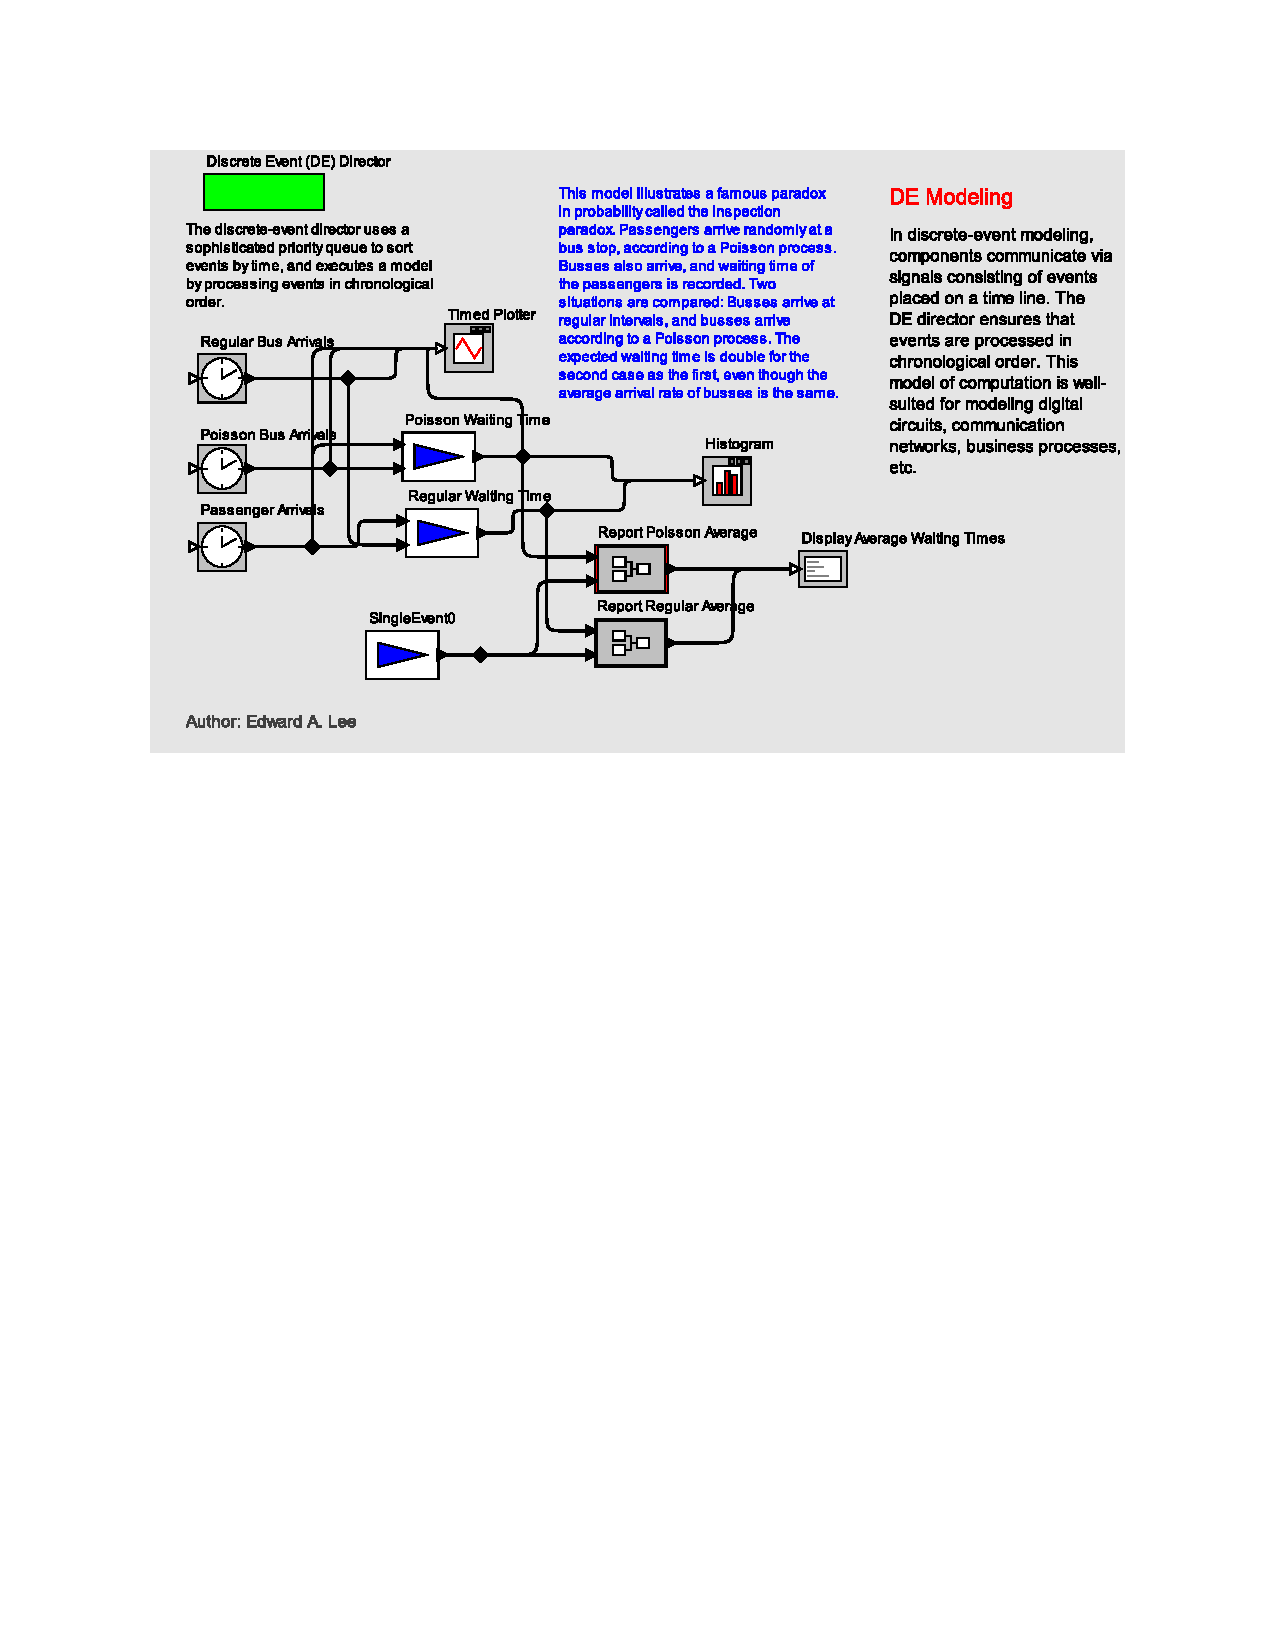
\includegraphics[width=3.5in]{figure.pdf}
  \end{center}

  \caption{\small Figure caption. To get a figure to span two
      columns, use the environment figure* rather than figure.}
  \label{fig-label}
\end{figure}


Suppose you wish to include a figure, like that in figure \ref{fig-label}.
The simplest mechanism is to install Adobe Acrobat, which includes
a ``printer'' called ``Acrobat Distiller.'' Printing to this printer
creates a PDF file, which can be included in a document as shown
here.  To include Ptolemy II models \cite{PtolemyVol1:04},
just print to the distiller from within Vergil and reference
the PDF file in your \LaTeX document.

There is a bit more work to do, however.
The file that is produced by the distiller represents
a complete page, not the individual figure.
You can open it in using Acrobat (version 5.0 or later),
and select Document $\rightarrow$ Crop Pages from the menu.
In the resulting dialog, check ``Remove White Margins.''
Save the modified PDF file in a file and then reference
it in the \LaTeX file as shown in this example.

An alternative is to generate EPS (encapsulated postscript),
but the process is much more complex and fragile.
I recommend using pdflatex and Adobe Acrobat.

\bibliographystyle{abbrv}
\bibliography{refs}
\end{document}
